\subsection{Dati e risultati}

\begin{figure}[b]
    \begin{circuitikz}[scale=0.8, transform shape]
    % tre rettangoli con rispettivi nodi
    \foreach \i/\text in {0/Contatore,3.2/DAC,6.4/Comparatore} {
        \draw 
        (\i,0) rectangle ++(2.2,2)
        (\i+1.1,1) node [scale=0.9] {\text}
                (\i,1)   node [right] (\text_in) {}
                (\i+2.2,1) node [left]  (\text_out){}
        ;
        }
        % collegamenti grossezza normale
        \draw
        (DAC_out.east) -- (Comparatore_in.west)
            (Comparatore_out.east) -- ++(0.5,0) -- ++(0,1.5) coordinate(A){}
            (Contatore_in.west) -- ++(-0.5,0) |- (A)
            (Contatore_in.west) ++(-0.5,-0.3) node{U/D}
        ;
        % collegamento spesso e grigio (bus)
        \draw[line width=3pt, gray]
    (Contatore_out.east) -- (DAC_in.west)
            (Contatore_out.east) ++(0.5,0) -- ++(0,-1.5) -- ++(0.5,0) node[right,black]{OUT}
        ;
        % triangolino e clock sotto contatore
        \draw
        (0,0) ++ (1,0) coordinate (C)
            (C) ++ (-0.2,0) -- ++(0.2,0.2) -- ++(0.2,-0.2)
            (C) -- ++(0,-0.5) -- ++(-0.5,0) node[left]{CLK}
        ;
        % V da comparare sotto al comparatore
        \draw
        (Comparatore_in.west) ++(1,-1) -- ++(0,-0.5) -- ++(-0.5,0) node[left]{$V\ped{COMP}$}
        ;
        % fine
    \end{circuitikz}
    \caption{Schema a blocchi del ADC.}
    \label{fig:schema_adc13}
\end{figure}

\begin{figure}[b]
    \small
    \begin{circuitikz}[scale=0.9, transform shape]
    % Collegamenti dell'opamp
        \draw
        (0,0) node (opamp)[op amp]{}
            (-0.4,0.75) -- node[near start, right]{4}  ++(0,1) node[above]{$-15V$}
            (0.4,0.25)  -- node[near start, right]{1}  ++(0,1) -- ++(0.5,0) node[rground]{}
            (-0.4,-0.75) -- node[near start, right]{8}  ++(0,-1) node[below]{$+15V$}
            (0,-0.5) -- node[near start, right]{5}  ++(0,-1) -- ++(0.4,0) -- node[near end, right]{6} (0.4,-0.25)
        ;
        % partitore a sx
        \draw
        (opamp.+) -- ++(-0.5,0) coordinate(psx) -- ++(-0.5,0) to[R, l=10<\kilo\ohm>] ++(-2,0) -- ++(-0.5,0) coordinate(cpart)
            (cpart) to[R, l_=5.6<\kilo\ohm>] ++ (0,2)  node[above]{$-15V$}
            (cpart) to[vR, l=5<\kilo\ohm>]  ++ (0,-2) node[rground]{}
        ;
        % retroazione, pull-up, e pezzettino sul -
        \draw (psx) -- ++(0,-2) -- ++(0.5,0) to[R, l_=10<\mega\ohm>] ++(2,0) -- ++(1,0) coordinate(DP);
        \path[name path=verticale]   (DP) -- ++(0,3);
        \path[name path=orizzontale] (opamp.out) -- ++(3,0);
        \draw[name intersections={of=verticale and orizzontale, by=x}]
        (DP) -- (x)
            (x) -- (opamp.out) node[above left]{7}
            (x) to[R, l_=1<\kilo\ohm>] ++(0,2) node[above]{$+5V$}
            (x) -- ++(0.5,0) coordinate(xs)
            (opamp.-) -- ++(-1,0) coordinate(MP)
            (opamp.-) node[above right]{3}
            (opamp.+) node[above right]{2}
        ;
        % tratteggio
        \draw
            (xs) -- ++(1,0) node[below, text width=2cm, align=center]{alla porta $\text{U}/\overline{\text{D}}$}
            (MP) -- ++(0,1) node[above, text width=2cm, align=center] {dal DAC}
        ;
        % fine
    \end{circuitikz}
    \caption{Schema circuitale del blocco di comparazione.}
    \label{fig:adc13}
\end{figure}

\paragraph{Analog to Digital Converter}

Il circuito in figura \ref{fig:schema_adc13} mostra il diagramma a blocchi del convertitore analogico
digitale (ADC) che abbiamo montato. I primi due blocchi sono un contatore e un convertitore digitale analogico,
ovvero il circuito costruito nella precedente esperienza (visibile in figura \ref{fig:ds_dac12}).
Questi due blocchi generano un onda a dente di sega. Il terzo blocco è un comparatore che compara il segnale
da leggere ($V\ped{COMP}$) con il dente di sega. Lo schema del comparatore è riportato in figura \ref{fig:adc13}.
L'ampiezza dell'onda a dente di sega è l'altezza massima del
segnale che il convertitore può leggere. Nel nostro caso l'intervallo di conversione andava da -4 V a 0 V.

Il comparatore è un semplice comparatore LM311 che confronta la tensione proveniente dal DAC08 (generatore del dente di sega)
con il segnale da leggere. L'LM311 è un comparatore open-collector e quindi è necessario collegare l'uscita con
una tensione a scelta mediante una resistenza di pull-up. Noi abbiamo collegato l'uscita del comparatore a una tensione 
di 5 V e l'entrata invertente all'output del DAC08 e quella non invertente al segnale da misurare.
In questo modo l'uscita dell'LM311 è un 1 logico se il segnale è più grande della tensione proveniente dal DAC08
altrimenti. Ora arriva l'idea geniale del circuito: l'uscita del comparatore è poi collegata con l'ingresso
U/D del contatore contenuto del primo blocco (si veda \ref{fig:ds_dac12}).

In pratica il circuito si comporta così: all'accensione il segnale è più alto dell'output del DAC08,
poiché quest'ultimo parte dalla tensione più bassa. L'output del comparatore è tale per cui il contatore
conta verso l'altro, facendo aumentare l'uscita del DAC08. Ad un certo punto l'output del DAC08 supera il
segnale in ingresso: in comparatore cambia stato e il contatore conta verso il basso, facendo tornare il
DAC08 sotto al segnale. Allora il comparatore cambia ancora la direzione del conteggio, e poi di nuovo, etc.
Il segnale del DAC08 oscilla attorno al valore del segnale analogico. Se il segnale analogico cambia questo
sistema seguirà l'andamento del segnale molto velocemente. È un cosidetto sistema di tracking.

\begin{figure*}[b]
    \centering
    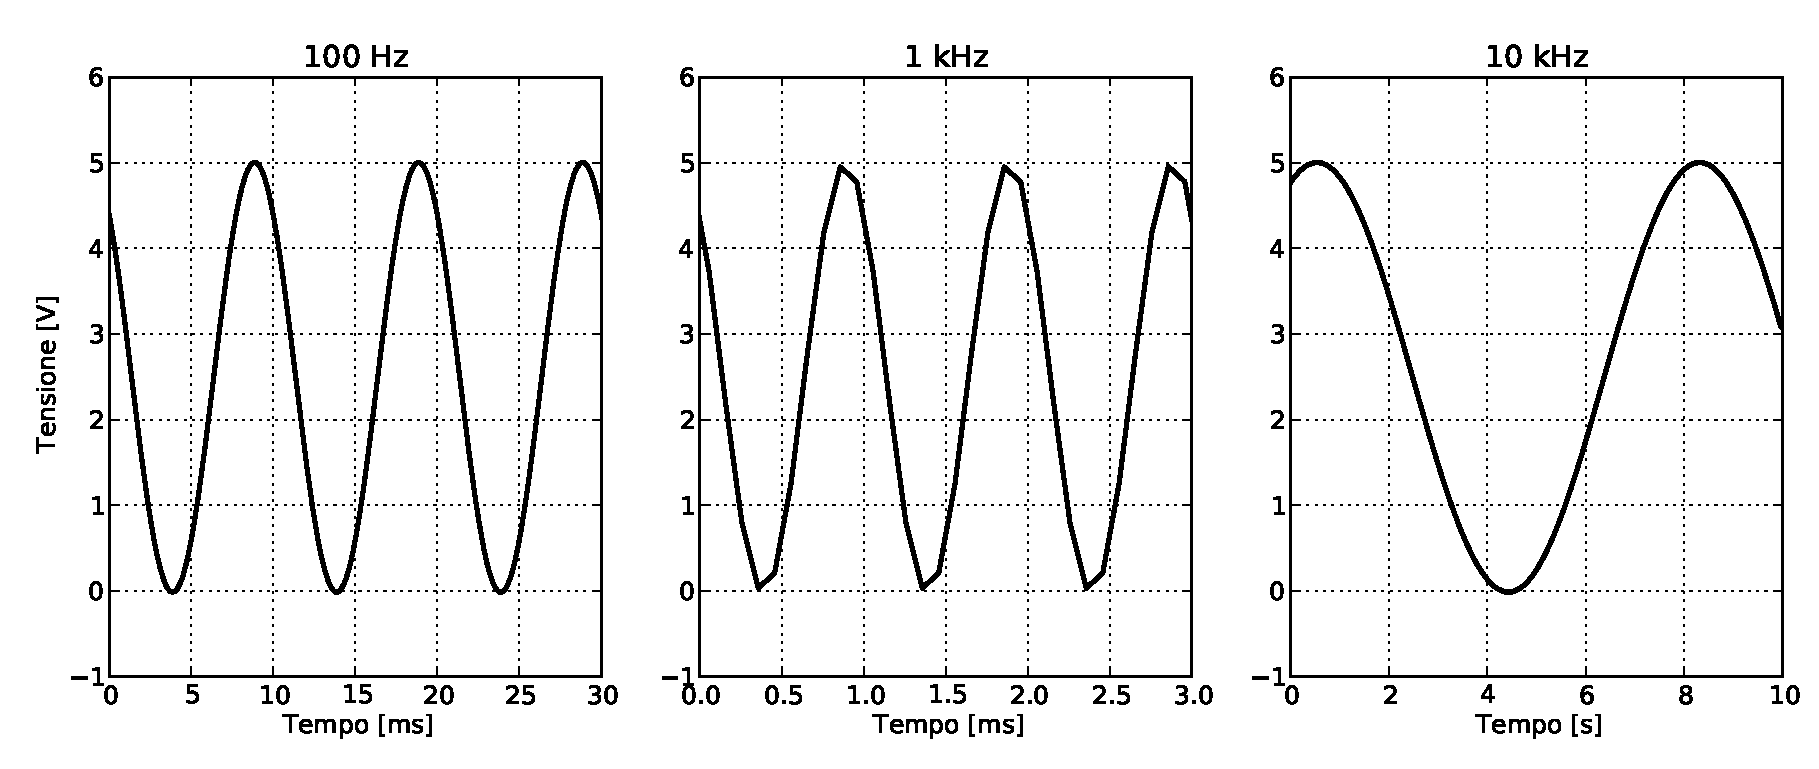
\includegraphics[width=\textwidth]{figure/camp.pdf}
    \caption{Campionamento di sinusoidi di varia frequenza. La frequenza di
        campionamento è stata mantenuta fissa a 10 kHz. Si vede molto bene il degrado
        della forma d'onda già con una frequenza di campionamento 10 volte superiore
        a quella dell'onda. Nel caso in cui la frequenza di campionamento
        e quella del segnale siano uguale è molto ben visibile il fenomeno
        dell'aliasing: un'onda di frequenza 10 kHz sembra un onda di frequenza
        di circa 0.1 Hz.}
    \label{fig:camp13}
\end{figure*}

Questo sistema rispetto ad altri simili ma senza tracking ha il,vantaggio di avere la stessa precisione
ma di essere più veloce, perché spesso i segnali cambiano lentamente e quindi il contatore parte da un valore vicino
a quello da misurare. Il valore digitale misurato è quindi l'uscita del contatore.

Per testare il circuito abbiamo usato un potenziometro ed una resistenza (figura \ref{fig:adc13}) per scegliere
e variare il segnale analogico, abbiamo usato una frequenza di clock bassa (100 Hz) per poter vedere il comportamento
del circuito e abbiamo usato la schedina con i LED per leggere il valore digitale in uscita. La tabella \ref{tab:adc13}
mostra alcune misure che abbiamo fatto. I risultati sono stati molto incoraggianti.

\begin{table}
    \begin{tabular}{l c c}
        \toprule
        Ingresso [V] & Valore letto & Equivalente [V] \\
        \midrule
        -4    & 227 & -4 \\
        -3.51 & 203 & -3.58 \\
        -3    & 173 & -3.05 \\
        -2.51 & 144 & -2.54 \\
        -2    & 116 & -2.04 \\
        -1.5  & 85  & -1.5 \\
        -1.02 & 57  & -1 \\
        -0.5  & 27  & 0.48 \\
        \bottomrule
    \end{tabular}
    \caption{Nella prima colonna è riportato il valore letto con l'oscilloscopio,
        nella seconda il numero che è stato letto nella schedina con i LED (convertito a decimale).
        L'ultima colonna riporta i valori della seconda colonna convertiti di nuovo a tensione per verificare
    il corretto funzionamento del circuito.}
    \label{tab:adc13}
\end{table}

\paragraph{Teorema del campionamento}

Per verificare e fare esperienza con i problemi relativi al campionamento, abbiamo campionato
alcuni segnali di diverso tipo mediante un computer. Nelle prove abbiamo mantenuto la frequenza
di campionamento invariata, variando la frequenza del segnale da campionare.

La figura \ref{fig:camp13} mostra un esempio di campionamento di un onda sinusoidale. La frequenza di
campionamento è stata mantenuta fissa a 10 kHz, mentre abbiamo misurato sinusoidi di 100 Hz, 1 kHz, 10 kHz, etc.
Evidentemente finché si sta al di sotto dei 5 kHz, come affermato dal teorema di Shannon, la sinusoide viene
campionata correttamente, anche se già a 1 kHz è visibile un degrado nella qualità del risultato. Andando invece a
frequenze vicine o superiori a quelle di campionamento, si mostra il fenomeno dell'aliasing, ovvero si ottengono
sempre sinusoidi, ma di frequenze completamente sbagiate, perché il campionamento non è abbastanza fitto.
Nel grafico si vede una sinusoide di 10 kHz che sembra avere una frequenza di 0.1 Hz!
